\documentclass[11pt]{article}
\usepackage{graphicx} % Required for inserting images
\usepackage[top=2.5cm, bottom=2.5cm, left=2.5cm, right=2.5cm]{geometry}
\usepackage[T1]{fontenc}
\usepackage{hyperref}
\usepackage[utf8]{inputenc}
\usepackage{multirow}
\usepackage{subcaption}
\usepackage{booktabs}
\usepackage{bookmark}
\usepackage{graphicx}
\usepackage{setspace}
\setlength{\parindent}{0in}
\usepackage{physics}
\usepackage{tikz}
\usepackage{tikz-3dplot}
\usepackage[outline]{contour} % glow around text
\usepackage{xcolor}
\usepackage{float}
\usepackage{makeidx}
\usepackage{fancyhdr}
\usepackage{pgfplots}
\usepackage{amsmath}
\pgfplotsset{compat=1.18}
\usepackage{caption}
\usepackage[english,catalan]{babel}
\setlength{\parskip}{11pt}
\usepackage{xcolor}
\usepackage{listings}


\title{\Huge\bfseries Cor:Cor \\[1ex] \Large}

\author{\begin{tabular}{c}
\textbf{GRUP C3} \\
Isaac Baldi (1667260)\\
Marcel López Freixes (1668323) \\
Eira Jacas García (1666616) \\
Núria Castillo Ariño (1669145)
\end{tabular}}

\date{data}

\begin{document}

\maketitle

En aquesta pràctica hem solucionat numèricament l'equació de difusió de la calor amb una font de calor externa. El problema es contextualitza en l'ablació cardíaca, que es una tractament mèdic que es basa en escalfar per efecte Joule el teixit biològic entre els ventricles del cor amb dos elèctrodes de polaritats oposades. Les condicions per a que el mètode sigui efextiu són que cap regió pot sobrepassar els 80 $^\circ$C, per evitar trombosis, i que la regió de teixit sa no superi els 50 $^\circ$C, quan comença la mort cel·lular. El nostre objectiu és trobar el temps màxim que podem aplicar una senyal de 40 V sense trencar aquestes condicions. Per fer-ho, estudiarem tres mètodes numèrics diferents: Euler explícit, Euler implícit i Crank-Nicolson i en compararem els errors numèrics amb la solució analítica per determinar quin es millor per solucionar el problema.

\section{Modelització del problema} 

L'equació diferencial que caracteritza el problema és

\begin{equation}
    c_v \rho \frac{\partial T}{\partial t} = \nabla(\kappa \nabla T) + P_{\text{ext}} \ ,
\label{eq: eq_inicial}
\end{equation}

on $P_{ext}$ representa la calor aportada al sistema per efecte Joule per unitat de temps i de volum. 

Si simplifiquem el sistema a un espai cilíndricament simètric, ens queda que

\begin{equation}
    c_v \rho \frac{\partial T}{\partial t} = \frac{\partial^2 T}{\partial x^2} + P_{\text{ext}} \ .
\label{eq: eq_inicial_cilindriques}
\end{equation}

Podem trobar el valor de $P_{ext}$ tenint en compte que la potència dissipada per efecte Joule en el cas d'un corrent altern, com el considerat en aquest problema, és $P_{Joule}=\frac{(V_{ef})^2}{R}=\frac{V^2 A \sigma}{2L}$, on A és la secció del cilindre al que hem simplificat el problema. Per tant, dividint pel volum del sistema obtenim que $P_{ext}=\frac{P_{Joule}}{AL}=\frac{V^2 \sigma}{2L^2}$.

\section{Normalització i condicions inicials i de contorn}

Dividint l'eq. \eqref{eq: eq_inicial_cilindriques} per $c_v\rho$ i definint $\lambda=\frac{P_{ext}}{\rho c_v}$, ens queda que

\begin{equation}
    \frac{\partial T}{\partial t} = \alpha \frac{\partial^2 T}{\partial x^2} + \lambda \ ,
\label{eq: eq_entre_rhocv}
\end{equation}

on $\alpha=\frac{k}{\rho c_v}$ és la difusivitat tèrmica.

Si dividim tot per $\lambda$ i definim $\hat{x}=\frac{x}{L}$, $\hat{T}=T \frac{\alpha}{\lambda L^2}$ i $\hat{t}=t\frac{\alpha}{L^2}$, aleshores

\begin{equation}
    \frac{\partial \hat{T}}{\partial \hat{t}} = \frac{\partial^2 \hat{T}}{\partial \hat{x}^2} + 1 \ .
\label{eq: eq_normalitzada}
\end{equation}

NO ENTENC QUE EM PREGUNTA DE LA NORMALITZACIO

Les condicions de contorn del problema són tals que als extrems del sistema o parets de la porció cilíndirca de teixit considerada, la temperatura es manté constant $T_c=36,5$ $^\circ$C. Pel que fa a les condicions incials, tenim que a $t=0$ s, la temperatura del teixit és $T_c=36,5$ $^\circ$C a tot arreu.

\section{Solució analítica}

Utilitzant la solució analítica proporcionada a l'annex del guió amb $q(x,t)=1$, obtenim

\begin{equation}
    f(\hat{x}, \hat{t}) = \beta + \frac{4}{\pi^3} \sum_{n=1}^{\infty} \frac{1 - e^{-(2n-1)^2 \pi^2 \hat{t}}}{(2n-1)^3} \sin\big((2n-1)\pi \hat{x}) \ ,
\label{eq: analitica}
\end{equation}

on $\beta=\hat{T}(T_c)$.


\section{Solucio numèrica: mètode d'Euler explicit}

Per aplicar el mètode numèric d'euler explicit utilitzem l'aproximació per la dreta de la primera derivada i la central per la segona, d'aquesta manera, definint $\gamma=\frac{\Delta \hat{t}}{\Delta \hat{x}^2}$, si el superindex és el temporal i el subindex l'espacial, ens queda que 

\begin{equation}
        \hat{T}_j^{i+1} = \gamma \left( \hat{T}_{j+1}^i - 2\hat{T}_j^i + \hat{T}_{j-1}^i \right) 
        + \hat{T}_j^i + \Delta \hat{t} \ ,
    \label{formuleta explicit}
\end{equation}

que amb les condicions inicials i de contorn definides, ens permet trobar per cada temps el valor del tamperatura a cada posició a partir de les temperatures trobades al temps anterior.

Si grafiquem les solucions numèriques corresponents a cada valor de $\gamma$ a $\hat{t}=t_a=0,025$, obtenim

\begin{figure}[hbt!]
    \centering
    \begin{subfigure}{0.5\textwidth}
        \centering
        \includegraphics[width=\textwidth]{euler_explicit_51_v2.png}
        \caption{$\gamma=0,51$}
    \end{subfigure}%
    \hspace{0.000001\textwidth}%
    \begin{subfigure}{0.5\textwidth}
        \centering
        %\includegraphics[width=\textwidth]{euler_explicit_49_25_v2.png}
        \caption{$\gamma=0.49$ i $\gamma=0,25$}
    \end{subfigure}
    \caption{Solució numèrica pel mètode d'Euler explicit pels diferents valors de $\gamma$ a $\hat{t}=t_a=0,025$.}
    \label{fig:resultats_explicit}
\end{figure}

on les línies verticals vermelles representen els extrems del teixit malalt.

Podem veure com per $\gamma=0,51$ la solució numèrica no té res a veure amb l'analítica, mentres que per $\gamma=0,49$ i $\gamma=0,25$ la solució numèrica és pràcticament igual a l'analítica. Això és degut a que el mètode d'Euler per l'equació de difusió amb una font d'energia externa només funciona o és estable per a un mallat o discretització tal que $\gamma \le 0,5$.

Pel que fa als errors numèrics de les solucions estables en aquest instant de temps, els representem al següent gràfic:

\begin{figure}[hbt!]
    \centering
    \includegraphics[width=0.5\textwidth]{errors_v2.png}  
    \caption{Errors numèrics de les solucions estables a $\hat{t}=t_a=0,025$.}
    \label{fig: error_explicit}
\end{figure}

COMPROVACIONS SI NO CONEIXESSIM LA SOLUCIO ANALITICA

\section{Solució numèrica: mètode d'Euler implícit}
En aquest mètode la derivada espacial de l'Eq. \eqref{eq: eq_normalitzada} es calcula aplicant l'aproximació pel centre, i la temporal per l'esquerra (aquí és on recau la diferència amb el mètode explícit).

Substituint les aproximacions de les derivades corresponentment a l'equació diferencial i aïllant $\hat{T}_j^n$,
\begin{equation}
    \hat{T}_j^n = \frac{\gamma \left( \hat{T}_{j+1}^n + \hat{T}_{j-1}^n \right) + \hat{T}_j^{n-1} + \Delta \hat{t}}{1 + 2\gamma}
    \label{Tnj implici}
\end{equation}
on $\gamma =\frac{\Delta \hat{t}}{\Delta \hat{z}^2}$. Remarquem que, per les condicions inicials i de contorn, $\hat{T}_j^1=\hat{T}_1^n=\hat{T}_N^n = \beta$, pel que són valors coneguts i no incògnites. Així doncs, per a $T^n_{2}$ i $T^n_{N-1}$ cal utilitzar expressions modificades.

Per la implicitat d'aquesta equació, la resolució numèrica del problema es planteja com un sistema lineal d'equacions algebraiques on les incògnites són les temperatures en cada posició, per a cada pas temporal $n$. L'Eq. \eqref{matriu implicit} és seva representació matricial, donada a la Secció \ref{subsec: matrius}.

Per a la resolució del sistema i l'anàlisi dels resultats, hem optat pel mètode de Gauss-Seidel, preferible respecte el de Jacobi després de comparar-los a la Secció \ref{subsec: comparacio jacobi gs}.

A la Fig. \ref{fig: implicit} es presenta una gràfica que mostra el perfil espacial de temperatures en el temps $t_a$. L'espai delimitat per les rectes vermelles representa la regió malalta. Addicionalment, a la Fig. \ref{fig: error implicit} es representa l'error absolut associat a cadascuna de les solucions numèriques respecte l'analítica. 

\begin{figure}[H!]
    \centering
    \begin{minipage}{0.45\textwidth}
        \centering
        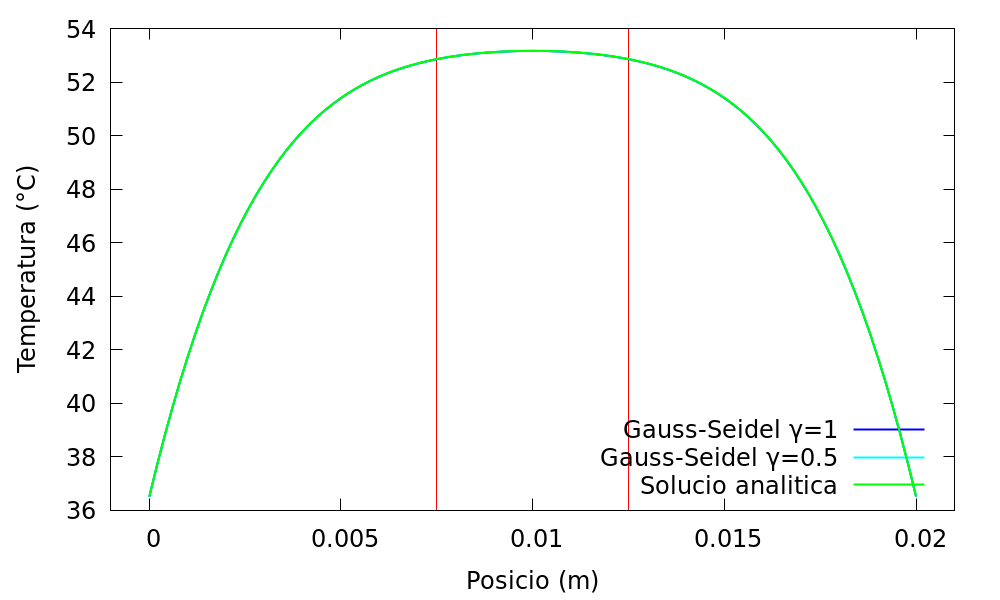
\includegraphics[width=\linewidth]{Implicit_N/implicit_grafica.png}
        \caption{Representació gràfica de les dues solucions numèriques junt amb la solució analítica.}
        \label{fig: implicit}
    \end{minipage}\hfill
    \begin{minipage}{0.45\textwidth}
        \centering
        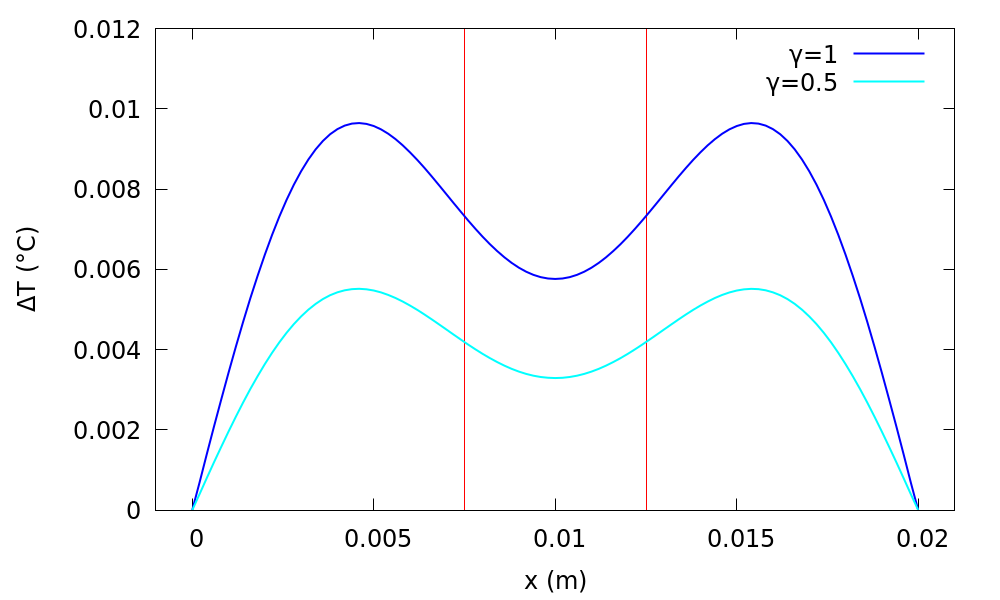
\includegraphics[width=\linewidth]{Implicit_N/error_implicit.png}
        \caption{Representació de l'error associat a cada solució.}
        \label{fig: error implicit}
    \end{minipage}
    \caption{Comparació de dues solucions numèriques obtingudes pel mètode d'Euler implícit per a $t=t_a$..}
    \label{fig:overall}
\end{figure}

En la Fig. \ref{fig: implicit}, les tres corbes pràcticament es solapen. Això indica que les solucions numèriques són gairebé idèntiques a l'analítica, posant de manifest l'alta precisió del mètode en ambdós casos.

Pel que fa la gràfica de l'error, es constata que aquest és molt petit (es manté inferior als 0,01 $^\circ$C) per a les dues solucions numèriques. No obstant això, permet identificar millor les diferències entre les dues solucions. S'aprecia que, per un valor de $\gamma = 0,5$, l'error és lleugerament menor que per $\gamma = 1$. Això suggereix que l'ús d'un pas temporal més petit millora la precisió.


\section{Solució numèrica: mètode Crank-Nicolson}

En aquest mètode numèric la discretització de la derivada temporal s'aproxima com en el mètode d'Euler explícit, l'Eq. \eqref{eq: derivada per la dreta}. En canvi, la segona derivada espacial com la mitjana de les dues posicions considerades a la discretització de la derivada temporal:

\begin{equation}
    \frac{\partial^2\hat{T}}{\partial \hat{z^2}} = \frac{1}{2}\frac{\hat{T}_{j+1}^n-2\hat{T}_{j}^n+\hat{T}_{j-1}^n}{\delta z}^2
    \label{mitjana segones derivades espacials}
\end{equation}

I ens acaba resultat l'expressió següent:
\begin{equation}
    \frac{\hat{T}_j^{n+1}-\hat{T}_j^{n}}{\Delta\hat{t}} = {\frac{1}{2}}(\frac{\hat{T}_{j+1}^{n+1}-2\hat{T}_j^{n+1}+\hat{T}_{j-1}^{n+1}}{\Delta\hat{z}^2}+\frac{\hat{T}_{j+1}^{n}-2\hat{T}_j^{n}+\hat{T}_{j-1}^{n}}{\Delta\hat{z}^2}) + 1
    \label{discretitzacio crank-nicolson}
\end{equation}

La resolució d'aquest problema també es planteja com un sistema d'equacions algebraiques, una per cada pas espacial, que cal resoldre iterativament per cada pas temporal $\hat{T}_j^n$. Com en el mètode d'Euler implícit, es parteix de les condicions inicials i es resol successivament per obtenir les temperatures dels passos següents de forma recursiva, aprofitant que els valors de $\hat{T}_j^{n-1}$ són coneguts del pas anterior.

El sistema es pot expressar en forma matricial per a cada pas $\hat{T}_j^n$, i per resoldre'l, utilitzem el mètode iteratiu de Jacobi.

\begin{equation}
  \begin{pmatrix}
    (\gamma - {1}) & {-}\frac{\gamma}{2} & {0} & {0} & \cdots & {0} \\
    {-}\frac{\gamma}{2} & (\gamma - {1}) & {-}\frac{\gamma}{2} & {0} & \cdots & {0} \\
    & \\
    \vdots & \vdots & & \ddots & & \vdots \\
    & \\
    {0} & {0} & \cdots & {-}\frac{\gamma}{2} & (\gamma - {1}) & {-}\frac{\gamma}{2} \\
    {0} & {0} & \cdots & {0} & {-}\frac{\gamma}{2} & (\gamma - {1}) \\
    \end{pmatrix}
    \begin{pmatrix}
        \hat{T}_{j=1}^{n+1} \\
        \hat{T}_{j=2}^{n+1} \\
        \vdots \\
        \hat{T}_{j=N-2}^{n+1} \\
        \hat{T}_{j=N-1}^{n+1} \\
    \end{pmatrix}
    =
    \begin{pmatrix}
        f_{j=1} +\frac{\gamma}{2}\hat{T}_{c} \\
        f_{j=2} \\
        \vdots \\
        f_{j=N-2} \\
        f_{j=N-1} +\frac{\gamma}{2}\hat{T}_{c} \\
    \end{pmatrix}
\end{equation}

\begin{center}
on $f = \frac{\gamma}{2}\hat{T}_{j+1}^{n} + (\gamma - {1})\hat{T}_{j}^{n} + \frac{\gamma}{2}\hat{T}_{j-1}^{n} + \Delta\hat{t}$
\end{center}

Per veure l'eficiència d'aquest mètode, compararem la solució analítica i la numèrica per a cada pas del 
mallat espacial per al temps $t_a = 0.025$ especificada en l'enunciat. Calculem l'error absolut entre les 
temperatures, que també ens servirà per comparar amb els altres dos mètodes numèrics que hem utilitzat.

\begin{figure}[hbt!]
    \centering
    \begin{subfigure}{0.3\textwidth}
        \centering
        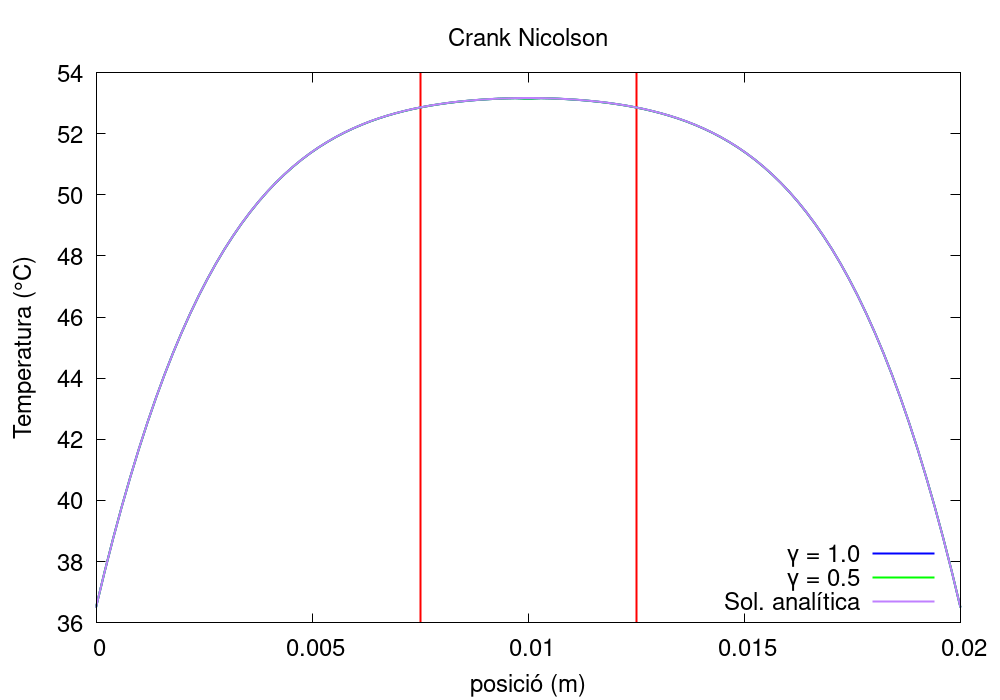
\includegraphics[width=\textwidth]{cranc2gamma.png}
        \caption{Solució Crank-Nicolson per diferents mallats.}
    \end{subfigure}
    \hspace{0.025\textwidth}
    \begin{subfigure}{0.3\textwidth}
        \centering
        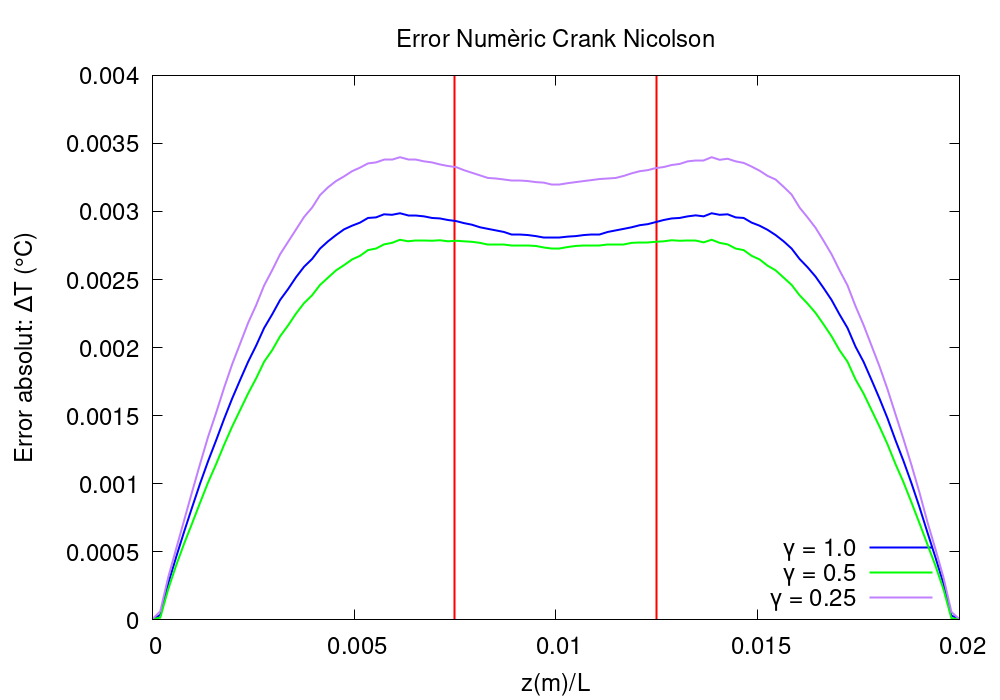
\includegraphics[width=\textwidth]{errcranc3gamma.png}
        \caption{Error numèric de Crank-Nicolson per diferents mallats.}
    \end{subfigure}
    \hspace{0.025\textwidth}
    \begin{subfigure}{0.3\textwidth}
        \centering
        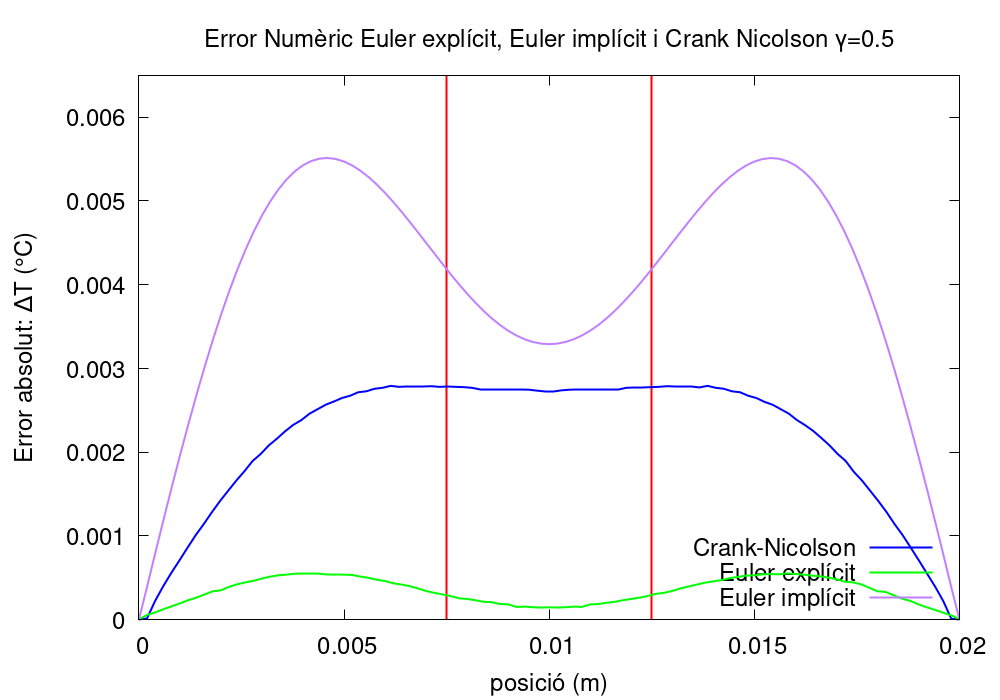
\includegraphics[width=\textwidth]{errtemp3met.png}
        \caption{Comparació Error numèrs 3 mètodes utilitzats.}
    \end{subfigure}
    \hspace{0.025\textwidth}
    \caption{Gràfics corresponents al mètode Crank Nicolson.}
    \label{fig:dues_imatges}
\end{figure}

Observant el gràfic de l'esquerra podem veure que l'error augmenta com més ens allunyem dels límits de l'interval espacial però que si ens aproximem al centre torna a disminuir. 
També podem observar que si reduim el tamany de l'interval del mallat, l'error es fa més petit. 
Això és perquè estem fent passos més petits en la discretització del temps. 
Al reduir el tamany dels passos ens apropem cada vegada més a la definició de diferencial i,per tant, l'equació discretitzada s'aproxima millor a l'equació diferencial que volem resoldre.

D'altra banda gràfics de la dreta, notem que la diferència de temperatura que presenta la solució numèrica de Crank és més gran que la que presenten els altres mètodes numèrics (Euler explícit i Euler implícit). 
La diferència entre el mètodes numèrics és el tipus de discretització que fem per a les derivades de l'equació diferencial. Així doncs, veiem que per aquest problema i per aquest interval d'espai i temps, aproximar la derivada segona com la mitjana de ens porta a una solució que s'allunya més de la solució analítica. 
Això podria ser perquè...SEGUIR

\section{Solució al problema}

Tenint en compte doncs que el mètode que millors amb un menor error numèric ha estat el mètode d'Euler explicit amb un mallat tal que $\gamma=0,25$, ens disposem a resoldre el problema amb aquest mètode i mallat. Si ens fixem en la solució numèrica trobada per $\gamma=0,25$ representada a la Fig. \ref{fig:resultats_explicit} (b), veiem com pel temps considerat la zona sana supera els 50 $^\circ$C, és a dir, que el temps que busquem és menor al corresponent a $\hat{t}=t_a=0,025$ i, per tant, peer solucionar el problema és suficient amb utilitzar el codi emprat en aquest cas imposant que en el pas temporal on les condicions que garanteixen l'eficiència del tractament es violin, s'aturi el mètode i es retorni el valor del temps que correspon a aquest pas. Fent això, obtenim un valor pel temps màxim que podem estar fent el tractament sense trencar les condicions que garanteixen la seva eficiència de $t=58,13$ s.

\begin{figure}[hbt!]
    \centering
    \begin{subfigure}{0.4\textwidth}
        \centering
        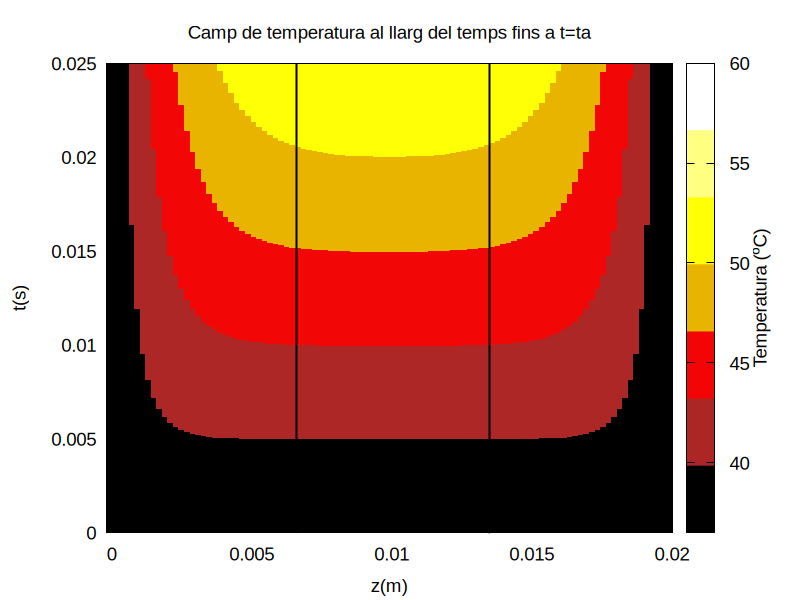
\includegraphics[width=\textwidth]{camp_ta.png}
        \caption{Veiem clarament que a t=ta hi ha parts del teixit sa per sobre de 50ºC.}
    \end{subfigure}
    \hspace{0.01\textwidth}
    \begin{subfigure}{0.4\textwidth}
        \centering
        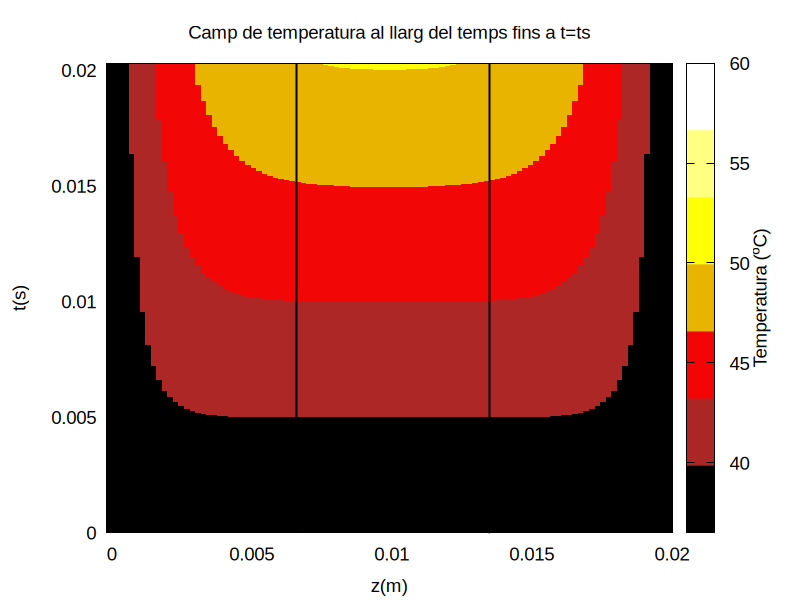
\includegraphics[width=\textwidth]{camp_ts.png}
        \caption{A t=ts just la marca de 50ºC toca els límits del teixit malalt.}
    \end{subfigure}


    \caption{Evolució del camp de temperatures amb el temps. Les línies horitzontals delimiten el teixit malalt.}
    \label{fig:dues_imatges}
\end{figure}


\section{Millora del model}

Per tal de millorar el model, podem tenir en compte la dependència de la conductivitat tèrmica amb la temperatura. La conductivitat tèrmica en materials dielèctrics com el teixit biològic no varia molt amb la temperatura ja que es fonamenta en la vibració de la xarxa (intercanvi de fonons) que per materials no cristal·lins depen poc amb la temperatura.$\footnote{\url{https://es.wikipedia.org/wiki/Conductividad}}
$ En conceqüència, per introduir la dependència de la conductivitat tèrmica amb la temperatura a l'equació, en faig l'expanció de Taylor fins a primer ordre:

$\kappa(T)\approx\kappa_0 +\kappa'_0T$

\begin{equation}
    C_v\rho\frac{\partial T}{\partial t} = \grad({\kappa (T)\grad{T}} )+ P_{ext}=\frac{\partial}{\partial x}(\kappa (T)\frac{\partial T}{\partial x})=\kappa_0\frac{\partial^2 T}{\partial x^2} + \kappa'_0\left(\frac{\partial T^2}{\partial x}\right)^2
\end{equation}
on $\kappa_0$ és la conductivitat tèrmica a la temperatura corporal, $T_c=36.5C^\circ$, i $\kappa'_0$ n'és la primera derivada a aquesta temperatura.



\section{Animació}
Un cop teniem els mètodes implementats hem representat els resultats amb dos gifs on es pot veure l'evolució del camp de temperatura en dues dimencions al llarg del temps. El nostre problema només depèn d'una dimenció espaial però per fer els gifs més representatiu del sistema d'electrodes que narra el problema, hem extès el camp de temperatures a una segona dimenció espaial. 
Per generara els gifs primer hem calculat el camp de temperatures en 100 temps equiespaiats i hem convertit aquestes dades en 100 fitxers txt. En segon lloc, hem plotejat les dades d'aquests fitxers amb una rutina de gnuplot obtenint 100 fotogrames. Per últim amb el programa ImageMagick hem seqüenciat els fotogrames per generar els gifs.
En els gifs veiem clarament com en els extrems dret i esquerra del camp, on hi hauria els electrodes, la temperatura es manté a la temperatura corporal i, en canvi, al mig, on hi hauria el teixit malalt, la temperatura va augmentant amb el temps. Al gif anomenat 'animacio1.gif' podem veure com la calor viatge a través del teixit, en el gif anomenat 'animacio2' podem veure com a partir del temps ts(=58s) hi ha parts del teixit sa que superen els 50$^\circ$C.



\begin{figure}[hbt!]
    \centering
    \begin{subfigure}{0.3\textwidth}
        \centering
        \includegraphics[width=\textwidth]{frame_000.png}
        \caption{frame 1}
    \end{subfigure}
    \hspace{0.01\textwidth}
    \begin{subfigure}{0.3\textwidth}
        \centering
        \includegraphics[width=\textwidth]{frame_050.png}
        \caption{frame 50}
    \end{subfigure}
    \hspace{0.01\textwidth}
    \begin{subfigure}{0.3\textwidth}
        \centering
        \includegraphics[width=\textwidth]{frame_100.png}
        \caption{frame 100}
    \end{subfigure}

    \caption{Tres frames representatius del gif animació 1}
    \label{fig:dues_imatges}
\end{figure}


\section*{Annexos}
\appendix

\section{Matrius dels sistemes d'equacions} \label{subsec: matrius}

Per al mètode d'Euler implícit, la representació matricial del sistema d'equacions en qüestió ve donada per la matriu següent.

\begin{equation}
  \begin{pmatrix}
    (2\gamma + {1}) & {-\gamma} & {0} & {0} & \cdots & {0} \\
    {-\gamma} & (2\gamma + {1}) & {-\gamma} & {0} & \cdots & {0} \\
    {0} & {-\gamma} & (2\gamma + {1}) & {-\gamma} & \cdots & {0} \\
    \vdots & \vdots & \vdots & \ddots & \vdots & \vdots \\
    {0} & {0} & \cdots & {-\gamma} & (2\gamma + {1}) & {-\gamma} \\
    {0} & {0} & \cdots & {0} & {-\gamma} & (2\gamma + {1}) \\
  \end{pmatrix}
  \begin{pmatrix}
    \hat{T}_{2}^{n} \\
    \hat{T}_{3}^{n} \\
    \vdots \\
    \hat{T}_{N-2}^{n} \\
    \hat{T}_{N-1}^{n} \\
  \end{pmatrix}
  =
  \begin{pmatrix}
    \Delta t + \beta\gamma + \hat{T}^{n-1}_2 \\
    \Delta t + \hat{T}^{n-1}_3 \\
    \vdots \\
    \Delta t + \hat{T}^{n-1}_{N-2} \\
    \Delta t + \beta\gamma + \hat{T}^{n-1}_{N-1} \\
  \end{pmatrix}
  \label{matriu implicit}
\end{equation}



\section{Comparació del mètode de Jacobi i el mètode de Gauss-Seidel}
\label{subsec: comparacio jacobi gs}

Els mètodes numèrics implícits són aquells en què no és possible aïllar una variable en funció d'altres variables únicament de passos anteriors. Entre els mètodes que hem utilitzat, l’Euler implícit i el Crank-Nicolson en són exemples.

La resolució numèrica d’aquests problemes es planteja com un sistema d’equacions algebraiques per a cada pas temporal. Utilitzar mètodes directes, com el de Gauss-Jordan, seria molt laboriós a causa de la dimensió del sistema. Per aquest motiu, es recorre a mètodes iteratius.

En aquesta assignatura se n'han presentat dos: el de Jacobi i el de Gauss-Seidel. El segon ofereix avantatges significatius, com un temps de càlcul més curt i menor requeriment d'emmagatzematge. No obstant això, considerem que el criteri rellevant per a seleccionar un mètode és el seu error. Per justificar la nostra elecció del mètode de Gauss-Seidel, hem comparat els dos mètodes en un cas concret.

En la Fig. \ref{fig: compar jacobi gs} es presenten, juntament amb la solució analítica, dues solucions numèriques del mètode d'Euler implícit amb $\gamma=1$ i en $t=t_a$: una obtinguda mitjançant el mètode de Jacobi (amb una tolerància entre passos de $10^{-7}$) i l'altra pel mètode de Gauss-Seidel (amb una tolerància de $10^{-3}$). A més, en la Fig. \ref{fig: error compar jacobi gs} es representa l'error absolut associat a cadascuna de les solucions numèriques respecte de l'analítica.

\begin{figure}[H]
    \centering
    \begin{minipage}{0.45\textwidth}
        \centering
        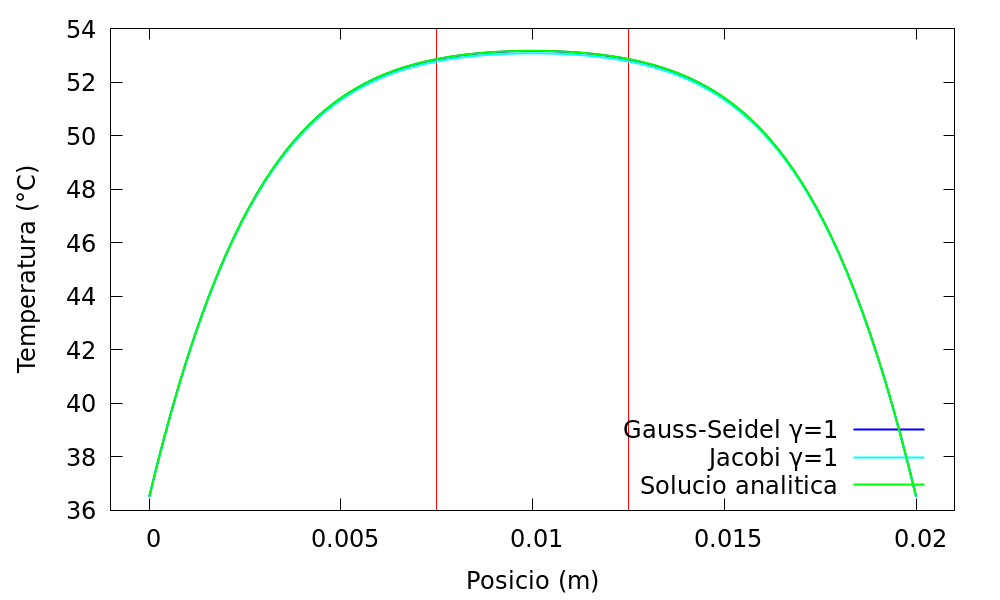
\includegraphics[width=\linewidth]{Implicit_N/implicit_grafica_comparacio.png}
        \caption{Representació gràfica de les dues solucions numèriques junt amb la solució analítica.}
        \label{fig: compar jacobi gs}
    \end{minipage}\hfill
    \begin{minipage}{0.45\textwidth}
        \centering
        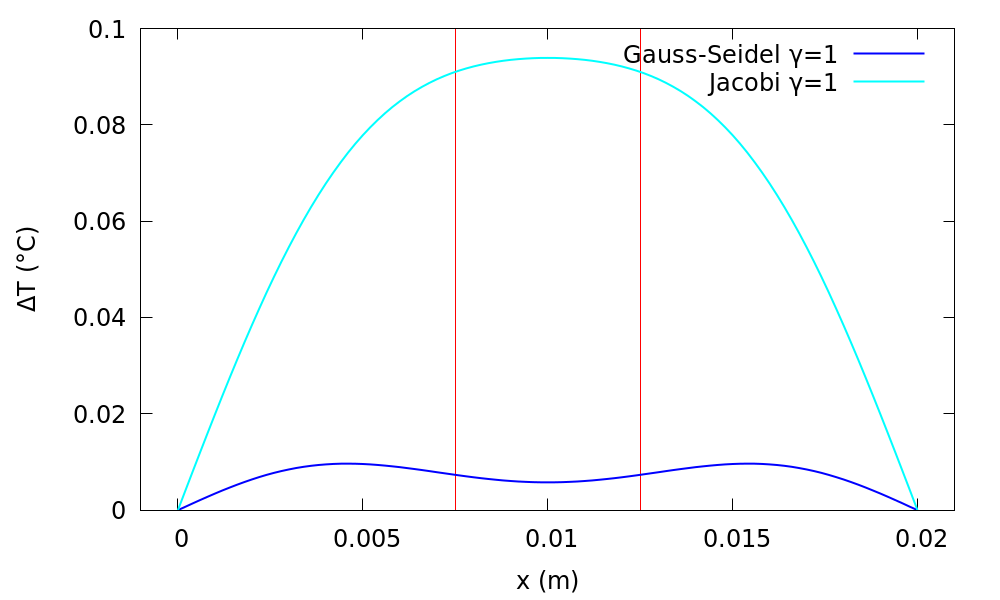
\includegraphics[width=\linewidth]{Implicit_N/error_implicit_comparacio.png}
        \caption{Representació de l'error associat a cada solució.}
        \label{fig: error compar jacobi gs}
    \end{minipage}
    \caption{Comparació del mètode de Jacobi i el de Gauss-Seidel per al mètode d'Euler implícit amb $\gamma=1$ i $t=t_a$.}
    \label{fig: comparacio jacobi i gs}
\end{figure}

En la Fig. \ref{fig: compar jacobi gs} s'aprecia que, a prop dels extrems, les solucions que proporcionen ambdós mètodes són molt similars a la solució analítica. Tanmateix, en la zona central la solució obtinguda amb el mètode de Jacobi presenta una lleugera desviació.

Aquest fet es reflecteix en la gràfica de l’error. Tot i que en tots dos casos l’error és petit (es manté inferior a 0,1 $^\circ$C), l'error en el mètode de Gauss-Seidel és significativament inferior.

En conclusió, hem escollit el mètode de Gauss-Seidel per resoldre el problema, ja que involucra menor error i millor eficiència computacional.



\end{document}


